\documentclass{TemplateLecture}

\renewcommand{\LectureName}{Lineare Algebra II}
\renewcommand{\ProfName}{Stefan Schwede}
\renewcommand{\Semester}{SoSe 2024}
\renewcommand{\mName}{Jan Malmström}

\begin{document}

\section{CW-Complexes}

The name abbreviates compact-Closure-Weak-Topology. They are \enquote{nice} classes of spaces for the purpose of homotopy theory/algebraic topology. They are build by successively attaching cells.

The \(n\)-cell is \(D^n = \set{x \in \IR^n: \abs{x} \leq 1}\). It may also be called \(n\)-balls or \(n\)-discs.
\(S^{n-1} = \partial D^n = \set{x\in \IR^n : \abs{x} = 1}\) is the \(n-1\)-Sphere.
See figure \ref{fig:exDn} for examples.

\begin{figure}
    \centering
    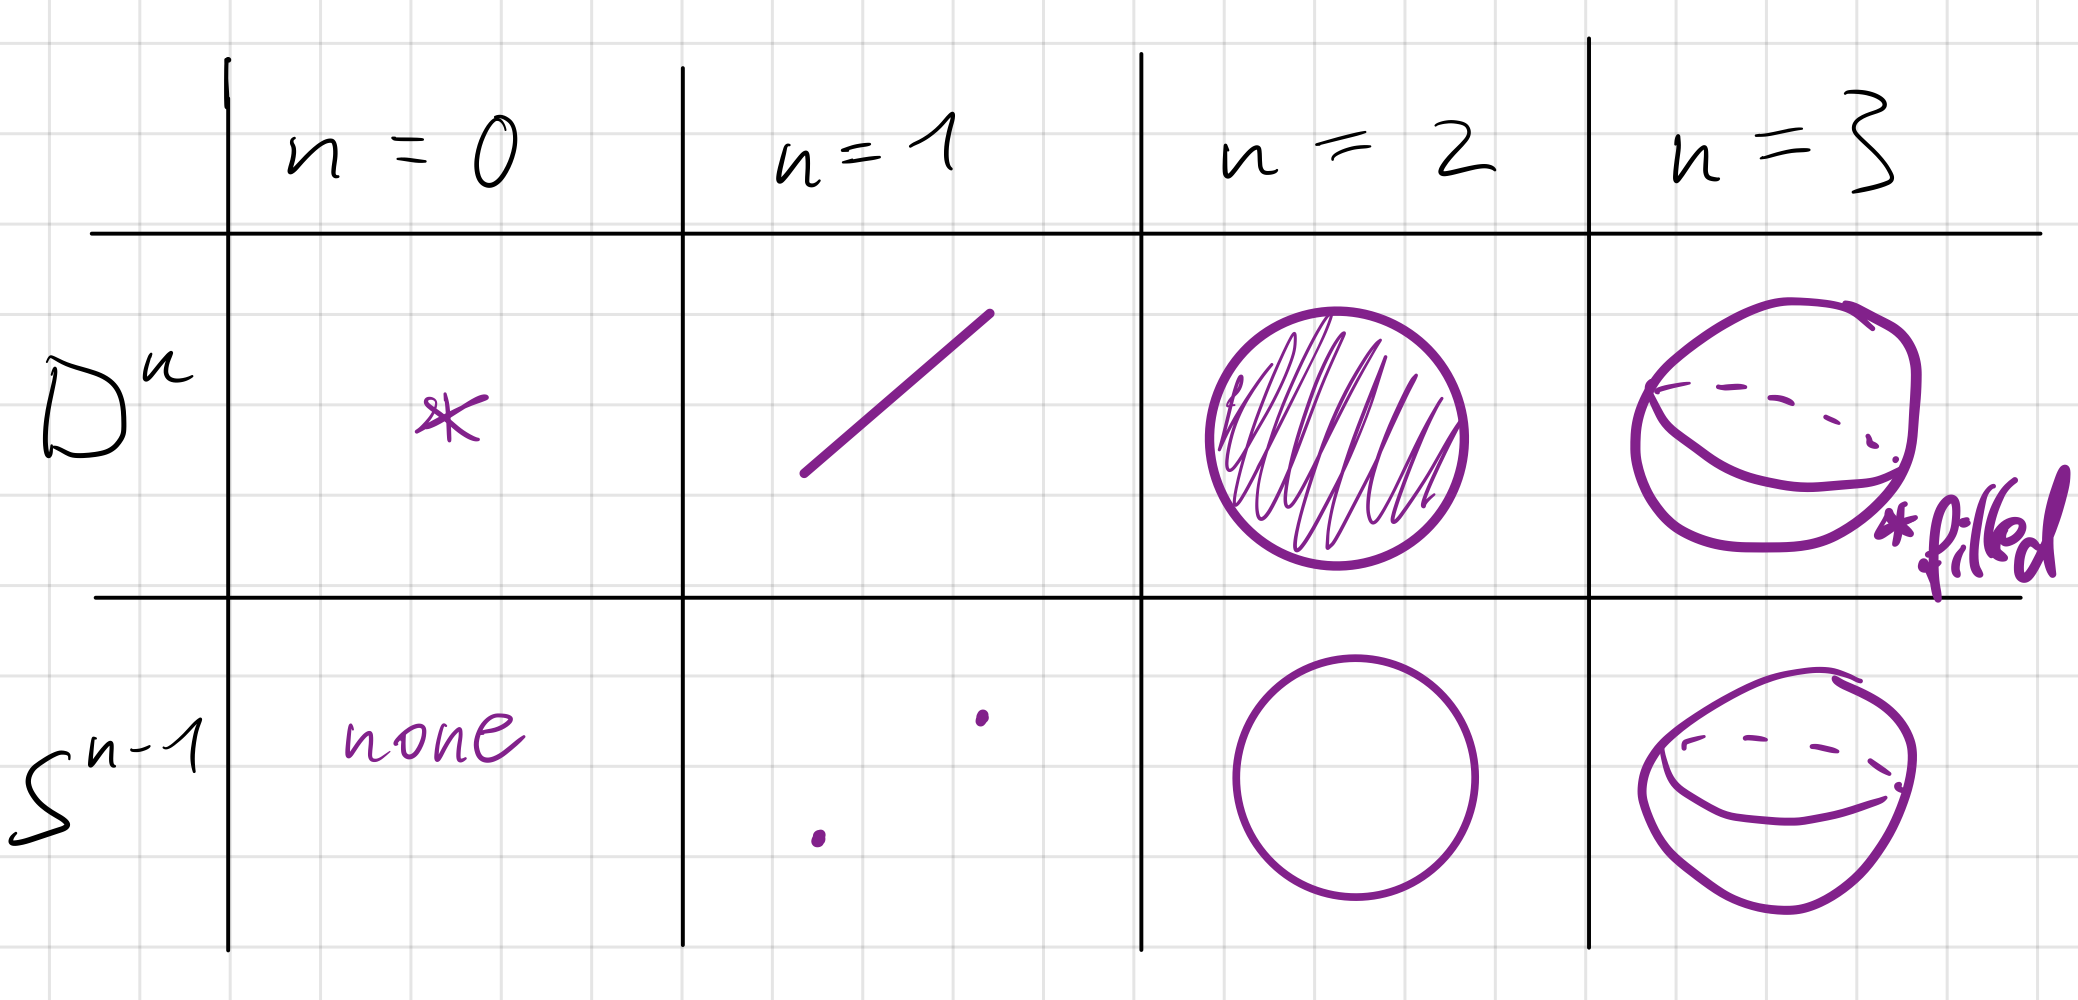
\includegraphics[width=0.8\linewidth]{pic/exDn.png}
    \caption{\(D^n\) and \(S^{n-1}\) for small \(n\)}
    \label{fig:exDn}
\end{figure}


\subsection{Definition}

\begin{construction}
    Let \(n \geq 0\), let \(f\colon S^{n-1} \to X\) be a continuous map, the \emph{attaching map}\index{Attaching map}. We form the quotient space
    \[X \cup_{f, \partial D^n} D^n = X \cup_f D^n = X \cup_{\partial D^n} D^n \coloneq X \amalg D^n/\sim\]
    where \(\sim\) is the equivalencce relation on \(X\amalg D^n\) genearted by \(\forall \; x \in S^{n-1}: f(x) \sim x\).
\end{construction}

\textbf{Terminology.} We say: \enquote{\(X\cup_f D^n\) is obtained by attaching an \(n\)-cell to \(X\) along \(f\)}.

\begin{bsp}
    \begin{itemize}
        \item \(X\cup_f D^0 = X \amalg D^0\)
        \item \(\set{*} \cup_{S^{n-1}} D^n = D^n/ \sim = D^n/ S^{n-1} \cong S^n\)
        
        In this example \(\sim\) identifies all of \(S^{n-1}\) to a point, which then is homeomorphic to \(S^n\)\footnote{supposed as known}.
        
        \item Remark, that the attaching map matters greatly. See figure \ref{fig:exAt}
        \[S^{n-1} \cup_f D^n \cong D^n \quad \text{with } f = \Id\colon S^{n-1} \to S^{n-1}\]
        \[S^{n-1} \cup_f D^n \quad \text{with } f \colon S^{n-1} \to S^{n-1} \text{ constant}\]
        \begin{figure}
            \centering
            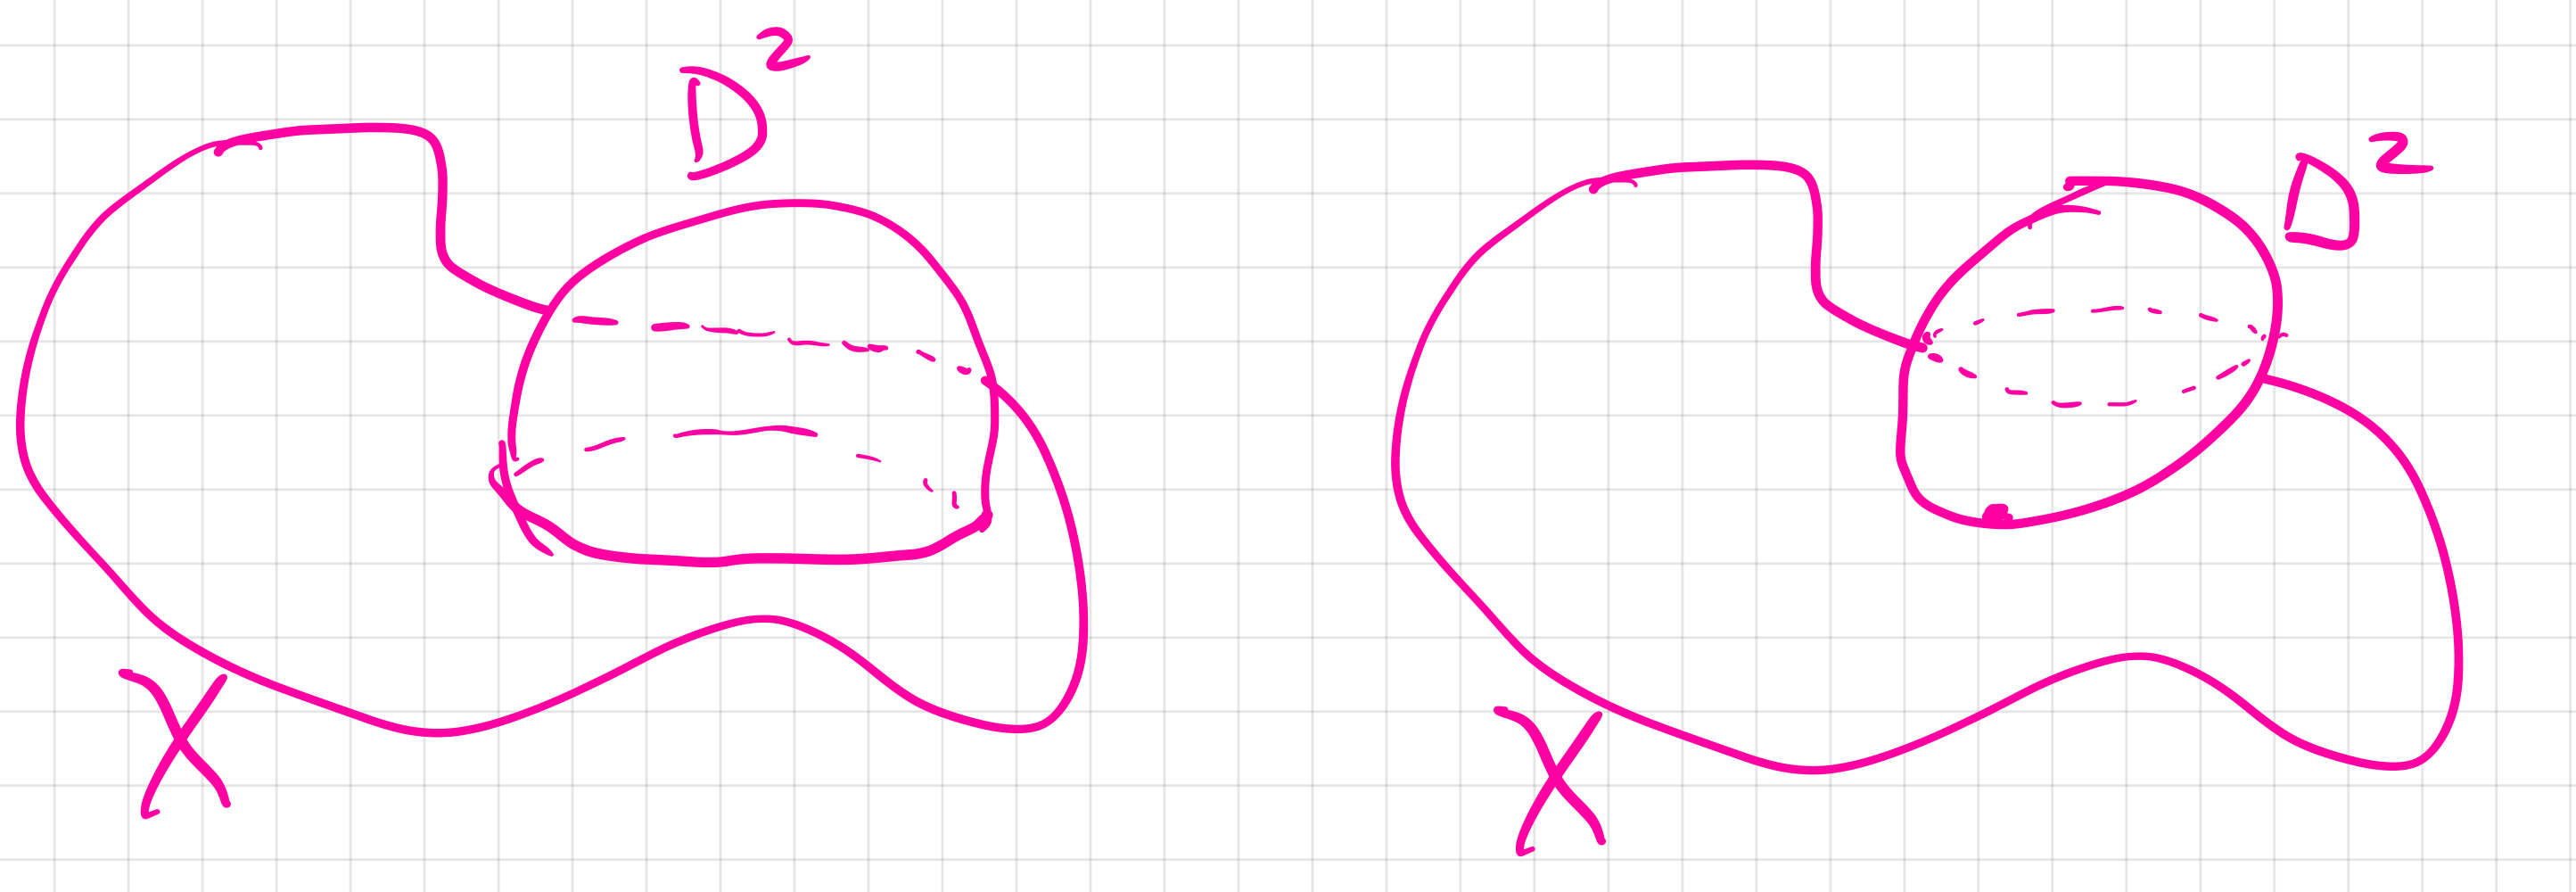
\includegraphics[width=0.8\linewidth]{pic/exAt.png}
            \caption{The attaching map influences how \(D^n\) is attached.}
            \label{fig:exAt}
        \end{figure}
    \end{itemize}
\end{bsp}

\subsubsection*{Simultaneous attachment of several cells}

Let \(J\) be an indexing\footnote{\enquote{indexing}does not carry mathematical meaning} set, considered as a discrete space (\(J = \emptyset\) is allowed).

Give \(J \times D^n\) the product topology, then
\[J \times D^n \cong \coprod_{j \in J} \set{j} \times D^n\text{\footnote{supposed as known}}\]
as a topological space. The \(\coprod\) represents the disjoint union topology.

It follows, that
\[\begin{tikzcd}
    \set{\text{continuous maps } f\colon J \times D^n \to X} \ar[d, phantom, "\cong", sloped] & f \ar[d, mapsto] \\
    \set{\text{J-indexed families of continuous maps } \set{f_j \colon D^n \to X}_{j \in J}} & f_j = f(j, \_)
\end{tikzcd}\]
We will identify them from now on.

\begin{defi}{}{}
    Let \(f \colon J\times \partial D^n \to X\) be a continuous map, the \emph{attaching map}\index{Attaching map}.
    \[X\cup_{f, J\times \partial D^n} J\times D^n = X \cup_f J\times D^n = X \cup_{J\times \partial D^n} J \times D^n \coloneq X \amalg J\times D^n /\sim\]
    where \(\sim\) is the equivalence relation generated by \(f(x) \sim x\) for all \(x \in J\times \partial D^n\).
\end{defi}



\textbf{Remark.} Write
\[p\colon X \amalg J\times D^n \to X\cup_f J\times D^n\]
for the quotient map. From the universal property of the qoutient map follows: Given maps \(g \colon X \to Y\) and \(\Psi_j \colon D^n \to Y\) such that \(g(f_j(x)) = \psi_j(x)\) for all \(j \in J, x \in \partial D^n\) there is a unique map \(\psi\colon X\cup_f J\times D^n \to Y\), such that
\[\psi \circ p = g + \coprod_{j \in J} \psi_j \colon X \amalg (J\times D^n) \to Y\]
and \(\psi\) is continuous iff \(g\) and all \(f_j\) are continuous.

Remeber the quotient-topology: A subset \(O\) in \(X \cup_f J\times D^n\) is open iff \(p^{-1}(O)\) is open in \(X \amalg J\times D^n\). This is equivalent to \(p^{-1}(O) \cap X\) is open in \(X\) and for all \(j \in J\) \(p^{-1}(O) \cap j \times D^n\) is open in \(D^n\).


\(X\) is a closed subspace of \(X\cup_f J\times D^n\) \(J \times \mathring{D^n}\) is an open subset of \(X\cup_f J\times D^n\)
\(X \cup_f J\times D^n\) is as a set (not as a space) the disjoint union of \(X\) and \(J\times \mathring{D^n}\).
We elaborate

\begin{proposition}
    \begin{enumerate}
        \item The composition
        \[\begin{tikzcd}
            X \ar[r] & X\amalg (J\times D^n) \ar[r, "p"] & X\cup_f J\times D^n
        \end{tikzcd}\]
        is a closed embedding (i.e. a closed injective map).
        \item The composition 
        \[\begin{tikzcd}
            J\times \mathring{D^n} \ar[r, hook, "incl"] & J\times D^n \ar[r] & X\amalg J\times D^n \ar[r, "p"] & X \cup_f J \times D^n
        \end{tikzcd}\]
        is an open embedding (i.e. injective and open)
        \item The underlying set of \(X\cup_f J\times D^n\) is the disjoint union of the image of \(X\) and \(J\times \mathring{D^n}\).
    \end{enumerate}
\end{proposition}

\begin{proof}
    Suppose \(M \subseteq X \amalg J\times D^n\) is saturated, i.e. \(M = p^{-1}(p(M))\). If \(M\) is saturated and open, then \(p(M)\) is open in \(X\cup_f J\times D^n\).
    \begin{enumerate}
        \item \begin{description}
            \item[\(n = 0\)] \(X\cup J\times D^0 = X \amalg J\times D^0\) is obvious.
            \item[\(n \geq 1\)] let \(r\colon D^n \to S^{n-1}\) be a map, such that \(r(x) = x\) for all \(x \in S^{n-1}\).This \underline{cannot} be done continuously.
            Define \(X \amalg J\times D^n \to X\) by \(x \mapsto x, (j,y) \mapsto r(y)\). This is compatible with the equivalence relation, so it descends to a (noncontinuous) map \(X \cup_f J\times D^n \to X\). This prooves injectivity.
            To show this is a closed map, we consider a closed subset \(A \subseteq X\). Then
            \(p^{-1}(p(A)) = A\amalg f^{-1}(A) \subseteq X\amalg J\times D^n\)
            \(\subset J\times \partial D^n \subset J\times D^n\) is closed in \(X \amalg J\times D^n\).
            So \(p(A)\) is closed in \(X\cup_f J\times D^n\).
        \end{description}
        \item All points in \(J \times \mathring{D^n}\) are their own equivalence classes, so the map is injective. To show that the map of 2. is open, we let \(B\) be an open subset of \(J\times \mathring{D^n}\). This is then also open in \(J \times D^n\). \(p^{-1}(p(B)) = \emptyset \amalg B\subset X\amalg J\times D^n\) open, so \(p(B)\) is open in \(X\cup_f J\times D^n\).
        
        \item I think this was prooven with a picture I didn't draw.
    \end{enumerate}
\end{proof}

\textbf{Exercise.} Let \(V_j\) be an open subset of \(D^n\) for every \(j \in J\), such that \(V_j \supset \partial D^n\). Show, that the set \(V = X \cup \bigcup_{j \in J} V_j\) is open in \(X\cup_f J\times D^n\).

From now on we often identify \(X\) with its image in \(X \cup_f J\times D^n\) and \(J\times \mathring{D^n}\) with its image in \(X \cup_f J\times D^n\)

\begin{defi}{Compactness}{}
    A space \(X\) is \emph{compact}, if it is Hausdorff (any two points can be separated by two disjoint open sets) and \emph{quasicompact} (any open cover has a finite subcover).
\end{defi}

\textbf{Remark.} Some literature defines compactness equivalent to quasicompactness. This lecture uses the definition that was given.

\begin{thm}
    Let \(f\colon J \times \partial D^n \to X\) be a continuous attacing map.
    \begin{itemize}
        \item If \(X\) is Hausdorff, then so is \(X \cup_f J\times D^n\).
        \item If \(X\) is compact and \(J\) is finite, then \(X \cup_f J\times D^n\) is compact.
        \item Let \(K\) be a quasicompact subset of \(X\cup_f J\times D^n.\) Then \(K\cap (\set{j} \times \mathring{D^n}) = \emptyset\) for almost all\footnote{mathematical term for all but finitely many.} \(j \in J\).
    \end{itemize}
\end{thm}

\begin{lem}
    There exists an open neighborhood \(V\) of \(X\) in \(X\cup_f J\times D^n\) and a continuous map \(r\colon V\to X\) that is the identity on \(X\). (\(X\) is a neighborhood retract inside \(X \cup_f J\times D^n\)).
\end{lem}

\begin{proof}
    picture.
    We take
    \(V = X\cup_{J\times \partial D^n} J\times (D^n\setminus {0})\)is open in \(X \cup_f J\times D^n\). We define \(r \colon V\to X\) by \(X\mapsto x, (j,z) \mapsto f(j, z/\abs{z})\)
\end{proof}

\begin{proof}of the theorem
    \begin{enumerate}
        \item \begin{description}
            \item[Case 1] \(x,y \in J\times \mathring{D^n}\). Since \(\mathring{D^n}\) is Hausdorff, so is \(J\times \mathring{D^n}\), so we can separate \(x\) and \(y\) by open disjoint subsets in \(J\times \mathring{D^n}\), Since \(J\times \mathring{D^n}\) is open in \(X \cup_f J\times D^n\), theses subsets are also open in \(X\cup_f J\times D^n\).
            \item[Case 2] \(x\in X, y \in \set{j} \times \mathring{D^n}\). We choose an \(y \in O_y \subset j \times D^n\) open \(j \times \partial D^n \subseteq V_j \subseteq j\times D^n\) s.t. \(O_j \cap V_j = \emptyset\).
            Then \(V\coloneq X\cup V_j \cup \bigcup_{k \in J\setminus\set{j}} D^n\) is open\footnote{by an exercise.} in \(X \cup_f J \times D^n\). \(V \cap O_j = \emptyset\), \(x \in V, y \in O_j\).
            \item[Case 3] \(x,y \in X\). Since \(X\) is Hausdorff, there are open subsets \(O_x, O_y\) of \(X\) with \(x \in O_x\), \(y \in O_y\), \(O_x \cap O_y = \emptyset\).
            We let \(V\) be an open subset of \(X \cup_f J \times D^n\) with a continuous retraction \(r\colon V\to X\), \(r\rvert_X = \Id_X\). Then \(x \in r^{-1}(O_x), y \in r^{-1}(O_y)\), \(r^{-1}(O_y), r^{-1}(O_y)\) are open, and disjoint.
        \end{description}
        \item If \(X\) is compact and \(J\) is finite, so is \(X\amalg J\times D^n = X \amalg \coprod_{j \in J} \set{j} \times D^n\) compact hence also the quotient space \(X \cup_f J\times D^n\) is quasi-compact. Hausdorff is inherted by \(1.\).
        \item Let \(K\) be a quasicompact subset of \(X \cup_{J\times D^n} J\times D^n\). We define subsets \(V_j\) of \(D^n\) for all \(j \in J\) as follows: If \(K \cap (j \times \mathring{D^n}) = \emptyset\), we set \(V_j = D^n\). If \(K \cap (j\times \mathring{D^n}) \neq \emptyset\), we choose a \(V_j\), that doen't contain at least one point of \(K\), is open, and contains \(\partial D^n\). Now \((X\cup_{j \in J} V_j) \cup \bigcup_{j \in J} \set{j} \times \mathring{D^n}\) is an open cover of \(X\). Since \(K\) is quasicompact, there is a finite subset \(L\) of \(J\) such that \(K \subset (X\cup_{j \in J} V_j) \cup \bigcup_{j \in L} \set{j} \times \mathring{D^n}\) much 
    \end{enumerate}
\end{proof}

\begin{bsp}
    Hawaiian Earrings
    \[H = H_1 \cup H_2 \cup H_3 \cup \dots = \bigcup_{i \geq 1} H_j\]
    where \(H_i = circle in \IR^2 of radius 1/i and center (0,1/i)\)

    picture. 
    with the subspace topology of \(\IR^2\). Is \(H\) obtained from \(\set{(0,0)}\) by attaching countably many 1-cells?

    It is not.
    Consider a continuous map \(\psi_j\colon D^l = [-1,1]\) such that is surjective and a homeomorphism of \([-1,1]/-1\sim 1\) onto  \(H_j \subset H\)
    %%hlep
    \(\set{(0,0)} \amalg \IN \times D^1 \to H\) is a continuous surjection%%Tikz
    \(\set{(0,0)} \cup_{\IN\times \partial D^1} \IN \times D^1\) is a continuous bijection.
    This is not a homeomorphism.

    Proof: Consider \(V = \set{(0,0)} \cup_{\IN \times \partial D^1} \IN \times [-1,0) \cup (0,1]\) open in 

    Complement of that is not closed.
\end{bsp}

\begin{defi}{}{}
    A relative CW-complex is a space \(X\) equipped with a sequence of closed subspaces
    \[A = X_{-1} \subseteq X_0 \subseteq X_1 \subseteq \dots \subseteq X_n \subseteq \dots \]
    such that
    \begin{enumerate}
        \item For every \(n \geq 0\) \(X_n\) can be obtained from \(X_{n-1}\) by attaching \(n\)-cells.
        \item \(X = \bigcup_{n \geq 0} X_n\) and \(X\) has the weak topology with respect to the sequences.
    \end{enumerate}

    more precise:
    There exists an index set \(J\), a continuous map \(f \colon J \times \partial D^n \to X_{n-1}\) and a homeomorphism \(\psi\colon X_{n-1} \cup_f J\times D^n \to X_n\) that is the identity on \(X_{n-1}\).
    a subset \(O\) of \(X\) is open in \(X\) is open in \(X\) iff \(O\cap X_n\) is open in \(X_n\) for all \(n \geq 0\) \(\Lra\) a subset \(C\) of \(X\) is closed in \(X\) iff \(C\cap X_n\) is closed in \(X_n\) for all \(n \geq 0\).
    \(\implies\) A map \(f\colon X\to Y\) is already continuous if \(f\rvert_{X_n}\colon X_n \to Y\) is continuous for all \(n \geq 0\).
\end{defi}

\begin{notation}
    We sometimes say \((X,A)\) is a relative \(CW-complex\) and leave the \(X_n\) implicit.
    For \(A = \emptyset\) \(X\) is called a absolute CW-complex, or just a CW-complex.

    The subspace \(X_n\) in a CW-complex is the \(n\)-skeleton.

    A relative CW-complex \((X,A)\) is finite-dimensional if \(X_n = X\) for some \(n \geq 0\).

    A relative CW-complex \((X,A)\) is finite, if there are only finitely many cells altogether.

    Once chosen a homeomorphism \(\psi\) as above, then the characteristic map  of the \(j\)-th \(n\)-cell is the composite \(D^n \to X_{n-1}\cup_{J\times \partial D^n} J \times D^n \to X_n \hookrightarrow X\) erste abb \(j, \_\), zweite \(\psi_n, cong\).

    \(X_j\rvert_{\mathring{D^n}} \mapsto X_j(\mathring{D^n})\) is a homeomorphism  ... , which is one path component of \(X_n \setminus X_{n-1}\). The restriction \(f_j \colon X_j\rvert_{\partial D^n} \to X_{n-1}\) is called the attacing map as before.
\end{notation}

Comment: The space \(X_n \setminus X_{n-1}\) is a disjoint union of open cells \(\mathring{D^n}\). So the indexing set could be taken as \(\pi_0(X_n\setminus X_{n-1})\).

For every path-component of \(X_n \setminus X_{n-1}\) there exists a homeomorphism \(f \colon \mathring{D^n} \to pathcomponent\), that extends to a continuous map \(\bar f \colon D^n \to X_n\).


\begin{example}
    Any discrete space is an absolute \(0\)-dimensional CW-complex.

    Let \(z \in S^n\) be any point. Then  the minimal CW-structure on \(S^n\) is \(X_{-1} = \emptyset, X_0 = \set{z} = X_1 = \dots = X_{n-1}\) \(X_n = X_{n+1} = \dots = S^n\). It consists of 1 \(0\)-cell and 1 \(n\)-cell. 

    \(S^n \cong D^n / \partial D^{n-1}\) \(z \leftarrow \partial D^{n-1}\)

    Example \(X = S^n\) \(n \geq 2\) Another CW-structure:

    picture

    \(X_{-1} = \emptyset, X_0 = X_1 = \dots = X_{n-2} = \set{(1,0,\dots, 0)}\) \(X_{n-1} = equator = \set{(x,0) : x \in S^{n-1}}\)
    \(X_n = X_{n+1} = \dots = S^n\)
    1 0 cell 1  \(n-1\)-cell 2 \(n\)-cells
    \(S^n \cong D^n \cup_{S^{n-1}} D^n\)

    Example: \(S^2\) 2 1 cell 2 2 cell 2 0 cell 
    picture

    Analog for \(S^n\) is a CW-complex with \(2\) \(i\)-cells for \(i = 0, \dots, n\).

    On \(S^1\) pick any finite subset \(A \subseteq S^1\). Then \(S^1\) has a CW-structure with \(X_{-1} = \emptyset, X_1 = A, X_2 = S^1\). n 0 cells n 1 cells.

    Any non-discrete space, that admits an absolute CW-structure admits uncountably many different CW-structures.

    Preview: The Euler characteristic of a finite absolute CW-comples is \(\chi(X) = \sum_{n \geq 0} (-1)^n \#n\text{-cells}\) does not depend on the CW-structure. We will eventually show this using singular homology. 
\end{example}

Then: Let \((X,A)\) be a relative CW-complex.
\begin{enumerate}
    \item If \(A\) is Hausdorff, then so is \(X\).
    \item If \(A\) is compact and \((X,A)\) is finite, then \(X\) is also compact.
\end{enumerate}

\begin{proof}
    Because \(X_{-1} = A\) is Hausdorff and \(X_n\) can be obtained from \(X_{n-1}\), by attaching cells, inductively \(X_n\) is Hausdorff for all \(n \geq 0\).
    Claim: Let \(O_n, P_n\) be open disjoint subsets of \(X_n\). Then there exist disjoint open subsets \(O_{n+1}, P_{n+1}\) of \(X_{n+1}\), such that \(O_n = O_{n+1} \cap X_n, P_n = P_{n+1} \cap X_n\).
    \begin{proof}
        Since \(X_{n+1}\) can be obtained from \(X_n\) by attaching \((n+1)\)-cells \(X_n\) is a neighborhood retract in \(X_{n+1}\), i.e. there are open neighborhood \(V\) of \(X_n\) in \(X_{n+1}\) and a continuous retraction \(r\colon V\to X_n\) with \(r \rvert_{X_n} = \Id\). We set \(O_{n+1} = r^{-1}(O_n), P_{n+1} = r^{-1}(P_n)\).

        Proof of the Hausdorff property: Let \(x,y \in X\) be disjoint points. Since \(X = \bigcup_{n \in \IN} X_n\). then for some \(n \geq 0\), \(x,y \in X_n\). Since \(X_n\) is Hausdorff, there are open, disjoint subsets \(O_n, P_n\) of \(X_n\) with \(x \in O_n, y \in P_n\). Inductiveleuse the claim to find open disjoint subsets \(O_m\), \(P_m\) of \(X_m\) for all \(m \geq n\), such that \(O_{m+1} \cap X_m = O_m, P_{m+1} \cap X_m = O_m\) for all \(m \geq n\). Then set \(O = \bigcup_{m \geq n} O_m, P = \bigcup_{m\geq n} PM\) disjoint subsets of \(X\) and open in \(X\) by the weak topology, as \(O\cap X_m = O_m\) open in \(X_m\).
    \end{proof} 

    Induction of \(n\) such that \(X_n\) is compact because \(X_n\) is obtained from \(X_{n-1}\) by attaching finitely many cells. Also \(X = X_n\)for sufficently large \(n\). So \(X\) is compact.
\end{proof}

Note: Suppose that \(X\) admits a CW-structure. Then the following are equivalent: \(X\) admits a finite CW-structure \(\Lra\) \(X\) is compact.

From now on standing assumption: the base \(A\) in a relative CW-complex \(X,A\) is Hausdorff.Then \(X\) is also Hausdorff.

Thus: Let \(X,A\) be a relative CW-complex.

\begin{enumerate}
    \item The closure of every open \(n\)-cell (\(=\) path component of \(X_n\setminus X_{n-1}\)) is compact.
    \item Let \(\chi\colon D^n \to X\) be a characteristic map for some \(n\)-cell, then  the image \(\chi(D^n)\) is the closure of the open cell \(\chi(\mathring{D^n})\)
    \item Let \(U\) be a subset of \(X\) s.t. \(A\subseteq U\). Suppose that the intersection of \(U\) with the closure of every cell is closed. Then \(U\) is closed in \(X\).
\end{enumerate}

Warning: the closure of a cell is not necessary a closed cell:

minimal CW-tructure on \(S^2\) open 2-cell \(S^2\setminus \set{z}\) closure \(= S^2 \neq D^2\).

\begin{proof}
    \begin{enumerate}
        \item By definition every open \(n\)-cells admits a characteristic map \(\chi\colon D^n \to X_n\) continuous s.t. \(\chi\rvert_{\mathring{D^n}}\) is a homeomorphis onto the open cells. Then \(\chi(D^n) \subseteq closure of open cell \chi(\mathring{D^n})\) so they are the same.
        %%hlep

        \item Let \(U\subseteq X\) be as in \(2\). It suffices to show that \(U\cap X_n\) is closed in \(X_n\) for all \(n \geq 0\) (weak topology). We argue by induction on \(n\).
        \(n = -1\) \(U\cap X_{-1} = U\cap A = A\) closed in \(A = X_{-1}\).
        \(n \geq 0\) We choose a homeomorphism \(\psi\colon X_n \cong X_{n-1} \cup_{J\times \partial D^n} J\times D^n\) that is the in?? on \(X_{n-1}\). We let \(p\colon X_{n-1} \amalg J\times D^n \to X_{n-1} \cup_{J\times \partial D^n} J\times D^n \psi \cong \to X_n\) be the ?? 

        \(p^{-1}(U\cap X_n = (U\cap X_{n-1}) \amalg \coprod_{j \in J} p^{-1}(U\cap closure of j-th n-cell))\) closed by hypothesis \(\subseteq X_{n-1} \amalg J\times D^n\)
        \(\implies\) \(U\cap X_n\) is closed in \(X_n\)
    \end{enumerate}
\end{proof}













\section{Higher homotopy groups}

\section{singular homology groups}

\end{document}